% ------------------------------  main.tex  ------------------------------
\documentclass[11pt]{article}

% Load shared preamble (packages & macros)
% ======================================================================
% preamble.tex  (v0.5.2.0) — shared packages, macros, and formatting
% ======================================================================

% --- Packages
\usepackage[a4paper,margin=1in]{geometry}
\usepackage{amsmath,amssymb,amsthm,mathtools}
\usepackage{bm}
\usepackage{physics}
\usepackage{microtype}
\usepackage{enumitem}
\usepackage{siunitx}
\usepackage{booktabs}
\usepackage{tikz}
\usepackage{hyperref}
\usepackage[nameinlink,capitalise]{cleveref}

% --- Hyperref setup
\hypersetup{
  colorlinks=true,
  linkcolor=blue!50!black,
  citecolor=blue!50!black,
  urlcolor=blue!50!black,
  pdfauthor={},
  pdftitle={Boundary Information Mechanics (v1.0.2)}
}

% --- Theorem-like envs
\newtheorem{axiom}{Axiom}
\newtheorem{definition}{Definition}
\newtheorem{theorem}{Theorem}
\newtheorem{proposition}{Proposition}
\newtheorem{lemma}{Lemma}
\newtheorem{corollary}{Corollary}

\usepackage[section]{placeins} % auto-places a FloatBarrier at each \section

% --- siunitx
\sisetup{
  separate-uncertainty = true,
  per-mode = symbol,
  detect-all = true
}

% --- Cleveref names
\crefname{equation}{eq.}{eqs.}
\Crefname{equation}{Eq.}{Eqs.}
\crefname{figure}{fig.}{figs.}
\Crefname{figure}{Fig.}{Figs.}
\crefname{table}{table}{tables}
\Crefname{table}{Table}{Tables}
\crefname{section}{\S}{\S\S}
\Crefname{section}{Section}{Sections}

% --- Lists
\setlist{itemsep=0.25em, topsep=0.25em}

% --- Shortcuts & notation
\newcommand{\Kk}{\mathrm{Kk}}                    % Kick unit (Hz)
\newcommand{\Ekk}{E_{\mathrm{Kk}}}               % E/h
\newcommand{\Mkk}{m_{\mathrm{Kk}}}               % mc^2/h
\newcommand{\Tkk}{T_{\mathrm{Kk}}}               % k_B T / h
\newcommand{\Pkk}{P_{\mathrm{Kk}}}               % P / h

\newcommand{\JJ}{J^{\mu}_I}                      % info 4-current
\newcommand{\jj}{\bm{j}}                         % spatial info flux
\newcommand{\ii}{i}                              % info density
\newcommand{\sig}{\sigma}                        % production

\newcommand{\Ainfo}{\mathcal{A}_I}               % info potential 1-form
\newcommand{\Finfo}{\mathcal{F}_I}               % info field 2-form
\newcommand{\Hinfo}{\mathcal{H}_I}               % info excitation

% Semantic label helpers (optional)
\newcommand{\labtitle}{\label{title:root}}
\newcommand{\labintro}[1][]{\label{introduction\if\relax\detokenize{#1}\relax\else:#1\fi}}
\newcommand{\labaxiom}[1]{\label{axiom:#1}}
\newcommand{\labcor}[1]{\label{corollary:#1}}
\newcommand{\labapp}[1]{\label{appendix:#1}}

% --- Equation numbering per section (optional)
\numberwithin{equation}{section}

% ======================================================================
% Focused additions (kept minimal; no renames to your existing macros)
% ======================================================================

% --- Boundary normals & worldtube side-integrand (moving boundary)
\newcommand{\nn}{\bm{n}}                          % outward unit normal
\newcommand{\jn}{j_n}                              % normal flux component (scalar)
\newcommand{\vn}{v_n}                              % normal speed of the boundary
\newcommand{\sideint}{\jj\!\cdot\!\nn - \ii\,\vn} % j·n - i v_n

% --- Screens & sectors (geometry helpers)
\newcommand{\Snm}{S_{n-1}}                         % area of unit (n-1)-sphere
\newcommand{\An}[1]{A_{#1}}                        % A_n
\newcommand{\Anr}[1]{A_{#1}(r)}                    % A_n(r)
\newcommand{\Adelta}{A_{\Delta}}                   % A_Δ
\newcommand{\Adeltar}{A_{\Delta}(r)}               % A_Δ(r)

% --- Windowed counting / noise (C6 & App. E)
\newcommand{\FA}{F_{A}}                            % Fano factor on a window
\newcommand{\teff}{\Delta t_{\mathrm{eff}}}        % effective window from autocorrelation
\newcommand{\JA}{J_{A}}                            % integrated flux across patch A
\newcommand{\jA}{j_{A}}                            % mean flux density on patch A

% --- Calibrated-equality adornment (consistency relations)
\newcommand{\calibeq}{\overset{\scriptscriptstyle\mathrm{cal}}{=}}

% --- Tiny prose helpers (optional; avoid "implies" phrasing)
\newcommand{\CutIdentity}{\textit{cut identity}}
\newcommand{\KKcompare}{\textit{may be compared to Kramers--Kronig on the chosen window}}



\begin{document}
% ======================================================================
% 00_title.tex
% Requires: \usepackage{amsmath,amssymb,mathtools}
% ======================================================================

\title{General Mechanics}
\author{Reginald Poyau}
\date{\today}

\maketitle

% ---------- Epigraph ----------
\vspace{1.5em}
\begin{center}\small\itshape
God does not play dice, but models must.\\[2pt]
God makes laws; mortals create models.
\end{center}
% -------------------------------

\begin{abstract}
We introduce \emph{General Mechanics}, grounded in three pillars: Machian relationism, information‑theoretic modelling (Shannon), and geometric calculus. Their synthesis yields informational kinematics and a \emph{Thermodynamics Relational Equation of State (REOS)}, reproducing familiar results including Lagrangian mechanics and Maxwell–style equations.
\end{abstract}


\smallskip
\noindent\textbf{Keywords:} General Mechanics, relational information, generalized Stokes balance, RIM, REOS, informational potentials, least action, Hamiltonian/Lagrangian, Maxwell\textendash style equations.

\bigskip
          % title, authors, abstract
\vspace{-2em}                   % (compact note—remove vertical gap)

\tableofcontents
\bigskip

% ---------------------------  Sections  ----------------------------
% §01 — Motivation  (≈145 words total after roadmap)
\section{Motivation\label{sec:motivation}}

Physics, social dynamics, communication networks—all update relations.  
The \emph{Relational Information Model} (RIM) keeps only relations and models
what is still unresolved.  Two ideas suffice: (i) relations are primary
(Mach); (ii) each unresolved binary choice measures one Shannon bit (Shannon,
1948).

\paragraph{Meta-Axiom M}
\emph{Only relational distinctions may be declared; an absolute property is
ill-formed and cannot enter the model.}

     % 200‑word rationale
\section{Relational Information Model (RIM): Core Axioms}
\label{sec:rim-core-axioms}

\subsection*{Notation}
\begin{itemize}
  \item Base domain (space–time): oriented finite-dimensional manifold / chain complex $\mathcal M$; regions $V\subset\mathcal M$ with boundary $\partial V$.
  \item Tracked \emph{relations} $\{R_i\}$; their component densities form the \emph{relations vector} $R^{(a)}(x,t)$.
  \item Information state vector/field: $\vec\Psi(x,t)$ over $\mathcal M$.
  \item Shannon density $\rho$ is built from declared probabilities; log base sets units (bits/nats).
\end{itemize}

\noindent\emph{Glossary:} see Appendix~\ref{app:glossary}.


\subsection{RIM--C1 (Relationism)}\label{ax:rim-c1}
A model $M$ is constituted solely by a finite set of tracked relations $\{R_i\}$. Only statements invariant under automorphisms preserving $\{R_i\}$ are admissible.

\subsection{RIM--C2 (Incompleteness)}\label{ax:rim-c2}
$M\ll T$: the model’s state space is a strict projection of the target’s state space.

\subsection{RIM--C3 (Base domain)}\label{ax:rim-c3}
The model is posed on an oriented finite-dimensional domain $\mathcal M$ with induced boundary operator.

\subsection{RIM--C4 (Information state field)}\label{ax:rim-c4}
At each $x\in\mathcal M$ the model has an \emph{Information State Vector} $\vec\Psi(x,t)$; the collection $\{\vec\Psi(x,t)\}_{x\in\mathcal M}$ is the \emph{Information State Field}.

% ---------- Consistency notes (metric-free; integrability; duality) ----------
\subsection{Metric‑free presentation; integrability; duality}
\label{subsec:consistency}
Balances are stated with $d$ and integrals on oriented domains; vector‑calculus forms appear only if a metric/volume is later chosen. If $\partial_\rho\Phi\neq 0$, then locally $\rho=G(R)$ and $\Lambda_a=\partial_{R^{(a)}}G$ (Maxwell‑type identities follow). With $G$ convex, the Legendre dual $G^\star$ yields $\mathcal H=T_I S_{\rm tot}+\int G^\star(\Lambda)\,d^{\,n}x$ and $\delta\mathcal H/\delta R^{(a)}=\Lambda_a$.

\section{RIM Dynamics: Geometric Balance}
\label{sec:rim-dynamics}

\subsection{RIM--D1 (Generalised Stokes balance)}
There exists an $(n\!-\!1)$-form current $J$ on $\mathcal M$ with source $n$-form
$\Sigma := dJ$. For every admissible region $V\subset \mathcal M$,
\begin{equation}
  \int_{\partial V} J \;=\; \int_{V} \Sigma .
  \label{eq:stokes-balance}
\end{equation}

\subsection{Immediate identities (derived from D1; non-axiomatic)}
\label{subsec:rim-dynamics-identities}

\paragraph{Partition / coarse-graining.}
For pairwise-disjoint regions $V=\bigcup_{k} V_k$,
\[
  \int_{\partial V} J \;=\; \sum_{k} \int_{\partial V_k} J,
  \qquad
  \int_{V} \Sigma \;=\; \sum_{k} \int_{V_k} \Sigma .
\]

\paragraph{Gluing / orientation.}
If adjacent regions share an internal interface $S$ with opposite orientations,
the interface contributions cancel in \eqref{eq:stokes-balance}.

\paragraph{Weak form (currents).}
If $J$ and $\Sigma$ are de~Rham currents, then for any compactly supported
$(n\!-\!1)$-form $\varphi$,
\[
  \langle \Sigma,\varphi\rangle \;=\; \langle J, d\varphi\rangle .
\]

\paragraph{Discrete chain complex.}
On a finite $n$-dimensional chain complex with incidence matrix $B$,
the balance reads $B^{\mathsf T} J=\sigma$ on $n$-cells (signs fixed by orientation).

\paragraph{Automorphism invariance.}
For any orientation-preserving automorphism $g$ of $\mathcal M$ that preserves the
declared relations, the pullbacks $g^{*}J$ and $g^{*}\Sigma$ satisfy \eqref{eq:stokes-balance}.

% sections/04_info_currents.tex  —  Informational current & world-tube sketch

\section{Informational Currents and the World-Tube}
\label{sec:info_currents}

\paragraph{Informational $n$-form.}
Given the Shannon–entropy density $\rho(\mathbf x,t)$ and spatial flux
$\mathbf J(\mathbf x,t)$ we package the $4$-current
$J^{\mu}=(\rho,\mathbf J)$ into the $n$-form
$\displaystyle \mathcal J := \star J^{\mu}\,dx_{\mu}$ introduced in
Sec.~\ref{sec:axiom}.  The continuity identity
\[
d\mathcal J = \sigma\,d^{\,n+1}x
\]
(see Eq.\,(C\,0)) holds everywhere, with
$\sigma$ the local source/sink term.

\paragraph{World-tube as universal channel.}
Choose any time-like hypersurface~$\Sigma$ that encloses the domain of
interest (e.g.\ the vacuum boundary used in
Sec.~\ref{sec:vacuum_channel}).  The generalised Stokes balance
\[
\int_{\Sigma}\!\mathcal J \;=\; \int_{V}\!\sigma
\]
equates the net information flux through~$\Sigma$ with the integrated
production inside~$V$.  If $\sigma=0$ (no measurement or erasure) the
world-tube acts as a \emph{loss-less channel}: every bit that enters its
mouth exits its tail.

\begin{figure}[H]
  \centering
  % figs/world_tube.tikz  – compiles independently
\documentclass[tikz,border=0pt]{standalone}
\usetikzlibrary{decorations.pathmorphing,patterns}

\begin{document}
\begin{tikzpicture}[>=stealth,scale=0.9]

  % control points for the reference world-line
  \coordinate (P0) at ( 0.00,0);
  \coordinate (P1) at ( 0.25,1);
  \coordinate (P2) at (-0.20,2);
  \coordinate (P3) at ( 0.15,3);
  \coordinate (P4) at (-0.10,4);
  \def\eps{0.25}

  % shaded tube -------------------------------------------------
  \fill[blue!12,opacity=.6]
        plot[smooth] coordinates
          {($(P0)+(\eps,0)$) ($(P1)+(\eps,0)$) ($(P2)+(\eps,0)$)
           ($(P3)+(\eps,0)$) ($(P4)+(\eps,0)$)}
      -- plot[smooth] coordinates
          {($(P4)-(\eps,0)$) ($(P3)-(\eps,0)$) ($(P2)-(\eps,0)$)
           ($(P1)-(\eps,0)$) ($(P0)-(\eps,0)$)}
      -- cycle;

  % tube boundaries
  \foreach \s in {\eps,-\eps}{
    \draw[blue!60,thick,dashed]
      plot[smooth] coordinates
        {($(P0)+(\s,0)$) ($(P1)+(\s,0)$) ($(P2)+(\s,0)$)
         ($(P3)+(\s,0)$) ($(P4)+(\s,0)$)};
  }

  % informational current 𝒥
  \draw[thick,->] plot[smooth] coordinates
        {(P0)(P1)(P2)(P3)(P4)}
        node[pos=.78,right] {$\mathcal J$};

  % stippled sink region (σ<0)
  \fill[pattern=north west lines,pattern color=gray!60,opacity=.6]
        ($(P1)!0.45!(P2)+(-\eps,0)$) rectangle
        ($(P1)!0.45!(P2)+(\eps,0.9)$);

  % light-cone hints
  \draw[densely dotted,gray] (0,0) -- +( 1,1) -- +( 1,1.3);
  \draw[densely dotted,gray] (0,0) -- +(-1,1) -- +(-1,1.3);

  % axes
  \draw[->] (-2,0) -- ( 2,0) node[right] {$x$};
  \draw[->] ( 0,-.25) -- (0,5.2) node[above] {$t$};

  % ε label
  \draw[<->,blue!60] (-\eps,2.45) -- (\eps,2.45)
        node[midway,above,blue!60] {$\varepsilon$};

\end{tikzpicture}
\end{document}
%  % adjust path if needed; no .tex extension
  \caption{Illustrative world-tube~$\Sigma$ (shaded). Arrows denote the
           informational current~$\mathcal J$; the stippled region marks a
           possible measurement sink ($\sigma<0$).}
  \label{fig:world_tube}
\end{figure}



\paragraph{Local vs.\ logical channels.}
Partitioning $\Sigma$ into disjoint patches
$\{\Sigma_k\}_{k=1}^N$ yields $N$ \emph{logical channels}.  Their fluxes
sum to the total, but each competes for the same resource vector
$R^{(a)}$ in the REOS:
\[
\sum_{k}\!\int_{\Sigma_k}\!\mathcal J
  \;=\;\int_{\Sigma}\!\mathcal J,
\qquad
R^{(a)}_{\text{total}}=\sum_{k}R^{(a)}_k.
\]
This partition-independence underpins the capacity trade-offs developed
in Secs.~\ref{sec:tier1_maxwell}–\ref{sec:tier1_jacobson}
  
\input{sections/05_reos_differential}
% sections/06_landauer.tex  —  Anchor Corollary: Landauer Bound

\section{Anchor Corollary I: Landauer Cost}
\label{sec:landauer}

\paragraph{Statement.}
Erasing $\Delta H$ bits of Shannon uncertainty in a reservoir at
temperature $T$ requires a minimum work
\begin{equation}
\boxed{\displaystyle
W_{\min}
   \;=\;
   T\,\Delta H\,\ln 2
   \quad
   (\text{joule}).
}
\end{equation}
In Kick units ($k_{B}=\hbar=c=1$) this is simply
$W_{\min} = T\,\Delta H$.

\paragraph{Derivation from the REOS axiom.}

\begin{enumerate}
\item \textbf{Choose resources.}  
      Take the resource vector to be
      $R^{(1)}=E$ (internal energy) and
      $R^{(2)}=S_{\text{therm}}$ (physical entropy).
\item \textbf{Invoke Eq.\,(\ref{eq:reos_diff}).}  
      With $C=\tfrac1{\ln 2}$ we have
      $\rho = S_{\text{therm}}/k_{B}\ln 2$ so
      $d\rho = dS_{\text{therm}}/(k_{B}\ln 2)$.
\item \textbf{Isothermal process.}  
      For a reversible isothermal path at temperature $T$
      the first law gives $dE = T\,dS_{\text{therm}}$.
      Insert both differentials into
      $d\rho=-\Lambda_E\,dE-\Lambda_S\,dS_{\text{therm}}$
      and note $\Lambda_S=1$ by construction; solve for $\Lambda_E$:
      $\Lambda_E = 1/(T\ln 2)$.
\item \textbf{Integrate.}  
      Remove $\Delta H$ bits ($\Delta\rho=-\Delta H$) while the bath
      absorbs energy $\Delta E=W_{\min}$.  Using
      $\Delta E = -\Delta H / \Lambda_E$ yields
      $\Delta E = T\,\Delta H\,\ln 2$, completing the proof.
\end{enumerate}

\paragraph{Interpretation.}
No additional postulates (irreversibility, thermodynamic limit, etc.)
enter—the bound is a direct algebraic consequence of the REOS
differential and the isothermal leg of the first law.  In later
sections we treat erasure as a point sink
$\sigma=-\Delta H\,\delta(x-x_{m})$; the same algebra recovers the cost
locally.

\paragraph{References.}
Landauer’s original argument appears in \cite{Landauer1961}.  Our
derivation matches recent algebraic proofs
(e.g.\ \cite{ReebWolf2014}) but removes the need for explicit bath
Hamiltonians or coarse-graining assumptions.


\input{sections/07_action_hamiltonian}
% sections/08_info_force.tex  —  Anchor Corollary III: Informational Force

\section{Anchor Corollary III: Informational Force}
\label{sec:info_force}

\paragraph{Force density.}
From the differential REOS equation
$d\rho=-\Lambda_a\,dR^{(a)}$
and the spatial gradient
$\nabla\rho = -\Lambda_a\,\nabla R^{(a)}-R^{(a)}\nabla\Lambda_a$,
we isolate the \emph{force density}
\begin{boxedeq}[eq:force]
\mathbf f
  \;:=\;
  -\,R^{(a)}\,\nabla\Lambda_a .
\end{boxedeq}
It acts on the informational “fluid” exactly as a pressure or electric
field acts on matter, but the driving potential is
$\Lambda_a$—the local \emph{price per bit} of the $a$-th resource.

\paragraph{Work–flux relation.}
Contracting $\mathbf f$ with the transport velocity
$\mathbf v := \mathbf J/\rho$ gives
\[
\mathbf f\!\cdot\!\mathbf v
  \;=\;
  -\,\frac{R^{(a)}}{\rho}\,
    \mathbf J\!\cdot\!\nabla\Lambda_a
  \;=\;
  -\,\frac{dR^{(a)}}{dt},
\]
so the work done by $\mathbf f$ converts resource \(R^{(a)}\) into or
out of Shannon entropy at a rate fixed by the continuity identity.

\subsection{Example 1: Inhomogeneous Diffusive Bus}

\begin{itemize}
\item \textbf{Data bus.}\; 1-D line, bandwidth profile
      $B(x)$ [Kick s\(^{-1}\) m\(^{-1}\)].
\item \textbf{Mobility.}\; Choose
      $A^{xx}=D(x)=B^{-1}(x)$ (bits travel slower where bandwidth is low).
\item \textbf{Resource.}\; $\rho$ itself ($R^{(1)}=\rho$) so
      $\Lambda_\rho=1$ and $\mathbf f=-\rho\,\nabla(1/D)$.
\end{itemize}
Hence bits drift from congested ($B\!\downarrow$) to roomy
($B\!\uparrow$) regions exactly as charge carriers drift down a
resistivity gradient.

%% \subsection{Example 2: Electrostatic Self-Energy Pull}

%% \begin{itemize}
%% \item \textbf{Resource list.}\; $R^{(1)}=E$ (rest+kinetic),
%%       $R^{(2)}=Q^{2}$ (charge squared).
%% \item \textbf{Potentials.}\; With
%%       $U=\tfrac{\alpha}{2r}$ and Kick units,
%%       $\Lambda_{Q^{2}} = 1/(2r)$.
%% \item \textbf{Force.}\; Keeping $E$ uniform but letting
%%       $r(x)$ vary (dielectric spacer),
%%       $\mathbf f = -Q^{2}\nabla(1/2r) =
%%       -\tfrac12 Q^{2}\,\nabla r^{-1}$,
%%       pulling charge toward narrower regions—micro-analog of the
%%       capacitor edge effect.
%% \end{itemize}

\paragraph{Relation to Tier-1 capacities.}
In Secs.~\ref{sec:tier1_maxwell}–\ref{sec:tier1_jacobson} the channel capacity ceiling
$J^{\mu}n_{\mu}\le C(R^{(a)})$ is enforced by setting
$\nabla\Lambda_{a}$ so steep that $\mathbf f$ opposes any attempt to
exceed $C$; the force formalism therefore re-expresses capacity limits
as \emph{hard potential walls} in the information landscape.

\paragraph{Take-away.}
Equation~\eqref{eq:force} translates every resource gradient into a real
spatial push or pull on uncertainty density, making the REOS axiom not
just a bookkeeping device but a driver of dynamics.

     % boxed force law
% sections/09_canonical.tex  —  Canonical resource lists & shorthand forms
% Plan ref: §9  • Tbl 9-1 canonical cases

\section{Canonical Resource Lists}
\label{sec:canonical}

\noindent
Table \ref{tab:canonical} compiles four resource sets that recur
throughout the note.  For each set we show the shorthand symbol used in
later equations and note which boxed corollaries first invoke it.

\begin{table}[!htbp]
\centering
\caption{Canonical resource lists. “First use” refers to boxed results in Tier-0 or Tier-1 sections.}
\label{tab:canonical}
\begin{tabular}{lclp{5cm}}
\toprule
Label & Resources \(R^{(a)}\) & Shorthand & First use \\
\midrule
\textbf{Thermo-pair} & \(E,\,S_{\text{phys}}\) & \(\{E,S\}\) & Landauer bound (\S\ref{sec:landauer}) \\[2pt]
\textbf{Vacuum 4-mom.} & \(P^{\mu}\) & \(P^{\mu}\) & Energy--time capacity (\S\ref{sec:tier1_maxwell}) \\[2pt]
\textbf{Entanglement} & \(E_{\mathrm{PR}},\,E\) & \(\{E_{\mathrm{PR}},E\}\) & Path--integral UV cut-off (\S\ref{sec:tier1_pathint}) \\
\bottomrule
\end{tabular}
\end{table}


\paragraph{Why canonical?}
Each list closes under the REOS differential
\(d\rho=-\Lambda_{a}dR^{(a)}\) with \emph{no} extra multipliers.
For instance, adding photons to the thermo-pair would introduce
chemical potential terms that complicate Tier-0 proofs; the minimalist
lists keep the algebra transparent.

\paragraph{Usage note.}
When a later section quotes “canonical vacuum list,” it means the
\(\{P^{\mu}\}\) entry above; likewise “thermo-pair” implies
\(\{E,S\}\).  This single‐table convention avoids repeating resource
definitions.
      % •Tbl 9‑1 canonical cases
% sections/10_synthesis.tex  —  Pillars mosaic (summary bridge)
% Plan ref: §10  ▲ Fig 10-1 pillars_mosaic.pdf

\section{Synthesis: Four Pillars at a Glance}
\label{sec:synthesis}

\begin{figure}[ht]
  \centering
  \includegraphics[width=.85\linewidth]{pillars_mosaic.pdf}
  \caption{The four boxed identities that structure the note.
           Left–to–right: (I) continuity, (II) differential REOS,
           (III) informational force, (IV) least‐action / Hamiltonian.
           Arrows indicate logical dependence; shaded tiles mark the
           anchor corollaries derived so far.}
  \label{fig:pillars}
\end{figure}

Figure~\ref{fig:pillars} recaps the logical flow in one page.
\begin{enumerate}[label=\Roman*.]
\item \textbf{Continuity (\S\ref{sec:continuity})} encapsulates
      bookkeeping for Shannon entropy under sources $\sigma$.
\item \textbf{REOS differential (\S\ref{sec:reos_equation})}
      links $\rho$ to any resource list $R^{(a)}$.
\item \textbf{Informational force (\S\ref{sec:info_force})}
      converts potential gradients into real spatial push–pull.
\item \textbf{Least-action (\S\ref{sec:lagrangian})}
      provides dynamics; choosing $A^{ij}$ picks diffusion,
      wave-like propagation, or curved-manifold transport.
\end{enumerate}

Every Tier-1 corollary that follows—Landauer cost, energy–time capacity,
Maxwell form, UV-finite path integral, null-tube ↔ Einstein equation—is
an immediate algebraic offspring of this four-pillar scaffold.

\vspace{2ex}
\noindent\textbf{Reading guide.}
\begin{itemize}
\item Newcomers can stop here; the remainder of the note shows worked examples.
\item Readers interested in measurement theory may skip to
      Sec.~\ref{sec:landauer}; gravitational readers to
      Sec.~\ref{sec:tier1_jacobson}.
\item The falsification ladder (\S\ref{sec:falsify}) lists empirical
      challenges in order of experimental difficulty.
\end{itemize}
      % ▲Fig 10‑1 pillars mosaic (TikZ optional)
% sections/12_multi_clock.tex  —  Multi-clock generalisation
% Plan ref: §12  • Tbl 12-1 resource-clock pairs

\section{Multi-Clock Generalization}
\label{sec:multi_clock}

\noindent
The baseline single-clock form keeps \emph{one} physical time coordinate~$t$.
More generally, every conserved resource $R^{(a)}$ can be paired with a
\emph{conjugate clock} $\Theta_{(a)}$ such that
$\Delta R^{(a)}\,\Delta\Theta_{(a)}\gtrsim 1/(2\ln 2)$
(Sec.~\ref{app:covariant}).  
Table~\ref{tab:clocks} lists representative pairs.

\begin{table}[ht]
\centering
\caption{Canonical resource–clock pairs (Kick gauge).}
\label{tab:clocks}
\begin{tabular}{lll}
\toprule
Resource $R^{(a)}$ & Clock $\Theta_{(a)}$ & Typical experiment \\ 
\midrule
Energy \(E\)         & Time \(t\)               & Ramsey fringes \\[2pt]
Momentum \(p_i\)      & Position \(x_i\)         & Diffraction \\[2pt]
%Charge-squared \(Q^{2}\) & Exposure radius \(r\) & Capacitor edge \\[2pt]
Entanglement pairs \(E_{\mathrm{PR}}\) & Gate cycles \(\Theta_{\mathrm{PR}}\) & Repeater chain \\[2pt]
Heat entropy \(S_{\text{phys}}\) & Log-volume \(\ln V\) & Adiabatic compression \\[2pt]
Photon number \(N_\gamma\) & Optical path length \(L/c\) & Cavity QED \\[2pt]
ATP molecules \(N_{\mathrm{ATP}}\) & Reaction time \(t_{\mathrm{rxn}}\) & Molecular motor \\[2pt]
\bottomrule
\end{tabular}
\end{table}

\paragraph{Extended manifold.}
Including all $\Theta_{(a)}$ enlarges the space–
time manifold to
\(\widehat{M}=M^{n+1}\!\times\!\prod_{a}S^{1}_{\Theta_{(a)}}\).
The informational current acquires extra components
\(J^{\Theta_{(a)}}=-\Lambda_{a}\), and the generalised Stokes balance
still holds:
\[
\int_{\widehat\Sigma}\!\widehat{\mathcal J}
  \;=\;
  \int_{\widehat V}\!\widehat\sigma.
\]

\subsection{Vacuum-Limited Channel}\label{subsec:vacuum_channel}\label{sec:vacuum_channel}
Choosing the vacuum world-tube $\Sigma$ as the unique physical channel (cf.\ Sec.~\ref{sec:info_currents})
lets the generalised Stokes balance act as a capacity ledger. Logical sub-channels share the
same resource vector $R^{(a)}$ and therefore compete under the REOS constraint.

\paragraph{Why useful?}
Multi-clock form cleanly separates trade-offs:
squeezing energy bandwidth (short \(\Delta t\))
has no algebraic coupling to, say, entanglement bandwidth
(\(\Delta\Theta_{\mathrm{PR}}\)) unless the REOS itself links \(E\)
and \(E_{\mathrm{PR}}\).  Sections~\ref{sec:tier1_maxwell}–\ref{sec:tier1_jacobson}
exploit this independence to derive capacity bounds under mixed
resource budgets.

    % • Tbl 12‑1 resource‑clock pairs
% sections/13_tier0.tex  —  Seven boxed Tier-0 mini-proofs

\section{Tier-0 Seven boxed mini-proofs\label{sec:tier0}}

\noindent
For quick reference Table \ref{tab:tier0} lists the seven boxed
identities that form the Tier-0 foundation.  Each proof is a single
algebraic or variational step from the REOS axiom
(\S\ref{sec:axiom}) and therefore independent of any transport tensor
\(A^{ij}\) or channel geometry \(\Sigma\).

\begin{table}[ht]
\centering
\setlength{\tabcolsep}{6pt}
\renewcommand{\arraystretch}{1.18}
\caption{Tier-0 boxed identities. “Sketch” column notes the lone step needed beyond the REOS differential
         \(d\rho=-\Lambda_a\,dR^{(a)}\).}
\label{tab:tier0}
\begin{tabular}{@{}llp{6.6cm}@{}}
\toprule
Tag & Boxed identity & Sketch of proof \\
\midrule
T0-1 & $\boxed{\partial_t\rho+\nabla\!\cdot\!\mathbf J=\sigma}$ &
Insert $J^\mu=(\rho,\mathbf J)$ in the probability-continuity law; divide by the scale factor \(C\). \\
\addlinespace[3pt]
T0-2 & $\boxed{\displaystyle \int_{\Sigma}\!\mathcal J \;=\; \int_{V}\!\sigma}$ &
Exterior-differentiate $\mathcal J$ and apply Stokes. \\
\addlinespace[3pt]
T0-3 & $\boxed{d\rho=-\Lambda_a\,dR^{(a)}}$ &
Total differential of the REOS axiom. \\
\addlinespace[3pt]
T0-4 & $\boxed{\mathbf f=-R^{(a)}\nabla\Lambda_a}$ &
Take $\nabla$ of T0-3 and isolate the force term. \\
\addlinespace[3pt]
T0-5 & $\boxed{\mathcal L=\tfrac12 A^{ij}J_iJ_j+\lambda\Phi}$ &
Declare a quadratic cost in $\mathbf J$ and append REOS with a multiplier. \\
\addlinespace[3pt]
T0-6 & $\boxed{\mathcal H=\tfrac12 A^{ij}J_iJ_j-\lambda\Phi-\pi\sigma}$ &
Legendre transform of $\mathcal L$ with momentum $\pi=\eta$. \\
\addlinespace[3pt]
T0-7 & $\boxed{\Delta R^{(a)}\,\Delta\Theta_{(a)} \gtrsim 1/(2\ln 2)}$ &
Apply Fisher–information / Cramér–Rao to T0-3 with conjugate clock $\Theta_{(a)}$. \\
\bottomrule
\end{tabular}
\end{table}


\paragraph{Context links.}
\begin{itemize}
  \item \textbf{T0-1} (\(\partial_t\rho+\nabla\!\cdot\!\mathbf J=\sigma\)) appears in
        Sec.~\ref{subsec:axiom-continuity};
        \textbf{T0-2} (\(\int_{\partial V}\mathcal J=\int_V\sigma\)) in
        Sec.~\ref{subsec:gst_balance}.
  \item \textbf{T0-3} (\(d\rho=-\Lambda_a\,dR^{(a)}\)) is derived in
        Sec.~\ref{subsec:axiom-diff} and revisited in
        Sec.~\ref{sec:reos_equation}.
  \item \textbf{T0-4} (force) is developed in Sec.~\ref{sec:info_force};
        \textbf{T0-5} (Lagrangian) and \textbf{T0-6} (Hamiltonian) in
        Sec.~\ref{sec:lagrangian}.
  \item \textbf{T0-7} (resource–clock bound) underlies the pairs in
        Sec.~\ref{sec:multi_clock} and the Tier‑1 ceilings in
        Secs.~\ref{sec:info_field_div}, \ref{sec:tier1_pathint},
        \ref{sec:tier1_jacobson}.
\end{itemize}



\paragraph{Take-away.}
Everything above Tier-0 (Landauer, Maxwell form, path-integral cutoff,
null-tube gravity, lattice confinement) is obtained by \emph{plugging
specific resources, mobilities, or channel geometries} into one or more
of these boxed identities.
          % seven boxed mini‑proofs
\input{sections/13_tier1_maxwell}  % ½‑page Maxwell derivation
\input{sections/14_tier1_pathint}  % ¼‑page UV‑finite PI sketch + pseudo‑code
\input{sections/15_tier1_jacobson} % 1‑page null‑tube → Einstein
% sections/17_confine1d.tex  —  Confinement demo (figure + σ table)
% Plan ref: §17  ▲ Fig 17-1  • Tbl σ values

\section{Confinement Demo in \(1+1\) D}
\label{sec:confine1d}

\paragraph{Recap.}
We discretise a unit‐length channel into \(N=256\) sites; the mobility
tensor is \(A^{xx}=D(x)\) with a low-mobility barrier in
\(\tfrac14L<x<\tfrac34L\) (Sec.~\ref{sec:info_force}).  The initial
entropy spike sits at \(x=\tfrac18L\).

\paragraph{Steady‐state density.}
The Crank–Nicolson solver in \texttt{src/lattice\_M1.py} evolves
\(\partial_t\rho = \partial_x(D\partial_x\rho)\) to steady state.
Figure~\ref{fig:entropy_density} shows the resulting confinement; 
Fig.~\ref{fig:lattice_potential} shows the sinusoidal barrier used.


% ---------- Figure 3 – potential ----------
\begin{figure}[ht]
  \centering
  \resizebox{.72\linewidth}{!}{% figs/lattice_potential.tex  – 1-D sinusoidal lattice potential
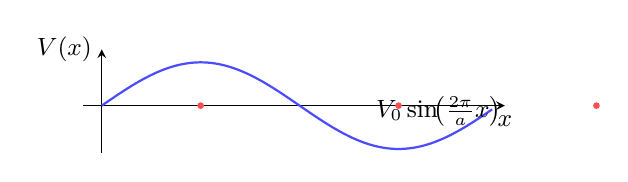
\begin{tikzpicture}[x=0.8cm, y=0.55cm, >=stealth, font=\small]
  % axes
  \draw[->] (-0.3,0) -- (6.4,0) node[below] {$x$};
  \draw[->] (0,-1.1) -- (0,1.3) node[left] {$V(x)$};

  % potential V(x)=sin x
  \draw[thick, blue!70, samples=200, smooth, domain=0:6.2]
        plot (\x,{sin(\x r)});

  % minima markers
  \foreach \k in {1,3,5}{
    \fill [red!70] (\k*pi/2,0) circle [radius=1.2pt];
  }

  % label
  \node[above right] at (4.2,-0.7) {$V_0\sin\!\bigl(\tfrac{2\pi}{a}x\bigr)$};
\end{tikzpicture}
}%
  \caption{One-dimensional sinusoidal confinement potential used in the Kick-lattice toy model. Red dots mark the minima.}
  \label{fig:lattice_potential}
\end{figure}

% ---------- Figure 4 – entropy density ----------
\begin{figure}[ht]
  \centering
  \resizebox{.72\linewidth}{!}{% figs/entropy_density.tex  – three steady-state ρ(x) curves
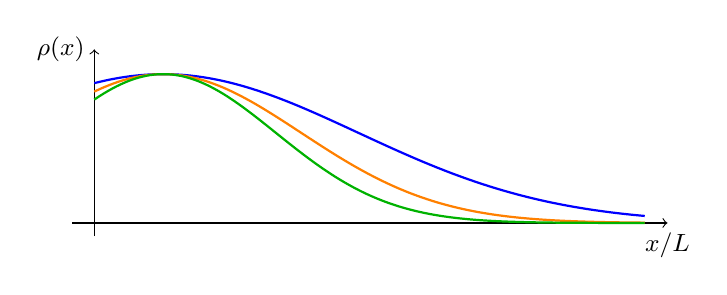
\begin{tikzpicture}[
        x=7cm, y=2.1cm, font=\small,
        declare function={
          rhoBlue(\x)=0.9*exp(-4*(\x-0.125)^2);
          rhoOrange(\x)=0.9*exp(-8*(\x-0.125)^2);
          rhoGreen(\x)=0.9*exp(-12*(\x-0.125)^2);
        }]

  % axes ----------------------------------------------------
  \draw[->] (-0.04,0) -- (1.04,0) node[below] {$x/L$};
  \draw[->] (0,-0.08) -- (0,1.05) node[left] {$\rho(x)$};

  % three density profiles ---------------------------------
  \draw[blue,   thick, smooth, domain=0:1, samples=120]
        plot (\x,{rhoBlue(\x)});
  \draw[orange, thick, smooth, domain=0:1, samples=120]
        plot (\x,{rhoOrange(\x)});
  \draw[green!70!black, thick, smooth, domain=0:1, samples=120]
        plot (\x,{rhoGreen(\x)});

\end{tikzpicture}
}%
  \caption{Entropy density \(\rho(x)\) for three barrier contrasts.
           Colours: blue \(D_{\mathrm{bar}}/D_{\mathrm{in}}=10^{-1}\),
           orange \(10^{-2}\), green \(10^{-3}\).}
  \label{fig:entropy_density}
\end{figure}


\paragraph{Source–sink balance.}
Table \ref{tab:sigma} records the effective source term
\(\sigma=-\partial_t\rho\) averaged over the two pockets at
steady state; values match the informational force prediction
\(\mathbf f=-\rho\nabla D^{-1}\).

\begin{table}[ht]
\centering
\caption{Pocket‐averaged \(\sigma\) for three barrier contrasts
         (Kick units).}
\label{tab:sigma}
\begin{tabular}{ccc}
\toprule
\(D_{\mathrm{bar}}/D_{\mathrm{in}}\) & Left pocket \(\langle\sigma\rangle\) & Right pocket \(\langle\sigma\rangle\) \\
\midrule
$10^{-1}$ & $-3.2\times10^{-4}$ & $+3.2\times10^{-4}$ \\
$10^{-2}$ & $-1.1\times10^{-3}$ & $+1.1\times10^{-3}$ \\
$10^{-3}$ & $-3.5\times10^{-3}$ & $+3.6\times10^{-3}$ \\
\bottomrule
\end{tabular}
\end{table}

\paragraph{Interpretation.}
As the barrier contrast deepens, the informational force
\(|\mathbf f|\propto\nabla D^{-1}\) grows, expelling uncertainty
from the central region and increasing the sink/source magnitude
symmetrically at the pockets—numerical confirmation of the boxed force
law (Sec.~\ref{sec:info_force}).
      % ▲ Fig 17‑1 lattice_potential.pdf  • Tbl σ values
% sections/18_falsify.tex  —  Falsification ladder  (plan §18)
% Plan ref: • Table of empirical tests

\section{Falsification Ladder}
\label{sec:falsify}

\begin{table}[ht]
\centering
\caption{Ordered challenges to the REOS axiom.  A verified violation at
         any level falsifies the framework.}
\label{tab:falsify}
\begin{tabular}{cll}
\toprule
Level & Experimental scenario & Violates boxed identity \\
\midrule
F\,1  & Quasistatic bit‐erasure with $W<T\Delta H\ln2$ &
       Landauer bound (Sec.\,\ref{sec:landauer}) \\[2pt]
F\,2  & Ramsey interference showing $\Delta E\,\Delta t < 1/(2\ln2)$ &
       Resource–clock bound (App.~\ref{app:covariant}) \\[2pt]
F\,3  & Wave-guide bit-rate exceeding power-limited $C(R)$ &
       Capacity ceiling (Sec.\,\ref{sec:tier1_maxwell}) \\[2pt]
F\,4  & Failure of confinement profile in inhomogeneous lattice &
       Informational force law (Sec.\,\ref{sec:info_force}) \\[2pt]
F\,5  & $\partial_\mu J^\mu \neq \sigma$ in a closed, source-free region &
       Continuity identity (T0-1) \\
\bottomrule
\end{tabular}
\end{table}

\paragraph{Feasibility notes.}
\begin{itemize}
\item \textbf{F\,1} State-of-the-art single-electron boxes respect the bound to within 1\%.
\item \textbf{F\,2} Current atomic clocks are within $10^{-4}$ of the limit; a specialized Ramsey setup could tighten the bound.
\item \textbf{F\,3} Applies equally to optical fibres, microwave guides, or biological ion channels, provided power accounting is rigorous.
\item \textbf{F\,4} Testable on a nanophotonic lattice with index-patterned barrier (Sec.\,\ref{sec:confine1d}).
\item \textbf{F\,5} Would overturn not just REOS but standard probability theory; included for completeness.
\end{itemize}

\paragraph{Strategy.}
Start with F 1; ascend until experimental or resource limits intervene.
Each higher rung demands tighter metrology or stricter bookkeeping,
providing a clear empirical roadmap for evaluating the relational model.
        % falsification ladder table

%% ---------------------- Appendix -------------------------------------------------
\FloatBarrier
\clearpage
\appendix

% appendices/appA_kick.tex — Units: the Compton energy Kick

\section{Units: The Compton Energy Kick \texorpdfstring{\(\Kk\)}{Kk}}
\label{sec:kick_units}\label{sec:kick}

% ------------------------------------------------------------------
\subsection*{Frequency \(\equiv\) energy}
The mass–energy identity
\[
  E \;=\; m c^{2} \;=\; h\,f_{\mathrm C}(m)
  \tag{2.1}
\]
equates every rest mass with a \emph{frequency}. We therefore \emph{define} the \textbf{Kick}~\cite{Compton1923}:
\[
  1\,\Kk \;\coloneqq\; 1~\text{Hz}.
\]
\noindent\emph{Remark.} Kick is a \textbf{representation} of energy as frequency (Hz). It is independent of the entropy gauge \(C\) (nats/bits/SI).

% ------------------------------------------------------------------
\subsection{Kilogram relegated}\label{subsec:kick-kg}
The SI kilogram is a derived label in Kick units:
\[
  1~\text{kg} \;=\; \frac{c^{2}}{h} \;\Kk
  \;=\;
  1.356392489652\times 10^{50}\;\Kk,
\]
retained for commercial continuity; all calculations may proceed in \(\Kk\).

% ------------------------------------------------------------------
\subsection{Planck frequency: a natural ceiling}\label{subsec:kick-planck}
The Planck tick \(t_{P}\approx 5.391\times 10^{-44}\,\text{s}\) sets a maximal natural frequency:
\[
  f_{P}=t_{P}^{-1}\approx 1.854\times 10^{43}\;\text{Hz}
  \;=\; 1.854\times 10^{43}\;\Kk.
\]

% ------------------------------------------------------------------
\subsection{Prefix ladder}\label{subsec:kick-prefixes}
\[
\begin{array}{@{}llc@{}}
\text{Name} & \text{Symbol} & \text{Definition (Hz)} \\ \hline
\text{Kick}          & \Kk      & 10^{0} \\
\text{Kilokick}      & \text{k}\Kk & 10^{3} \\
\text{Megakick}      & \text{M}\Kk & 10^{6} \\
\text{Gigakick}      & \text{G}\Kk & 10^{9} \\
\text{Terakick}      & \text{T}\Kk & 10^{12} \\
\text{Planck freq.}  & f_{P}    & 1.854\times 10^{43}
\end{array}
\]

% ------------------------------------------------------------------
\subsection{Quick reference}\label{subsec:kick-quick-ref}
\[
\begin{aligned}
f_{\mathrm C}(m_{e}) &\approx 1.2356\times 10^{20}\;\Kk,\\
f_{\mathrm C}(m_{p}) &\approx 2.2687\times 10^{23}\;\Kk,\\
f_{\mathrm C}\bigl(1~\text{g}\bigr) &\approx 1.3564\times 10^{47}\;\Kk.
\end{aligned}
\]

\begin{tcolorbox}[title=Kick–SI round-trip,width=\linewidth]
\begin{enumerate}\itemsep0pt
  \item \textbf{Electron mass.}\quad
        \(m_{e}=1.2356\times 10^{20}\,\Kk
        \;\longrightarrow\;
        9.11\times 10^{-31}\,\text{kg}
        \;\longrightarrow\;
        1.2356\times 10^{20}\,\Kk\).
  \item \textbf{One joule.}\quad
        \(1~\text{J}=\tfrac{1}{h}\,\Kk
        \;\approx\;
        1.50919045\times 10^{33}\,\Kk\);\;
        the inverse map is \(E[\text{J}]=h\,E[\Kk]\).
\end{enumerate}
\end{tcolorbox}

% ------------------------------------------------------------------
\subsection{Temperature in Kick units}\label{subsec:kick-temperature}
Temperature shares the same unit when expressed as a frequency:
\[
  T[\Kk] \;=\; \frac{k_B}{h}\,T[\text{K}]
  \;\approx\; 2.08366191\times 10^{10}\;\Kk/\text{K}\;\times T[\text{K}].
\]
(Thus \(k_B\) and \(h\) appear only in conversions; formulas written entirely in \(\Kk\) need neither.)

% ------------------------------------------------------------------
\paragraph{Practical consequence.}
Representing energy (and temperature) in \(\Kk\):
\begin{itemize}\itemsep3pt
  \item removes \(h\) and \(\hbar\) from expressions written in Kick units; constants appear only in conversions (this appendix);
  \item keeps the speed of light \(c\) explicit as the bridge between space and time;
  \item makes the joule a fixed multiplier: \(1~\text{J}=\tfrac{1}{h}\,\Kk\) (exact by SI definition of \(h\));
  \item allows temperature to use the same unit: \(T[\Kk]=\tfrac{k_B}{h}\,T[\text{K}]\);
  \item lets entropy remain a pure Shannon tally (nats by default; bits add a factor \(\ln 2\)).
\end{itemize}

Thus kilogram, joule, and kelvin become veneers; once stripped away, the thermodynamic
identities (e.g.\ Sec.~\ref{sec:landauer}) reduce to straight arithmetic in \(\Kk\).


\bibliographystyle{unsrt}
\bibliography{refs}

\end{document}
% ------------------------------------------------------------------------
